% !TEX TS-program = pdflatex
% !TEX encoding = UTF-8 Unicode

% This is a simple template for a LaTeX document using the "article" class.
% See "book", "report", "letter" for other types of document.

\documentclass[11pt]{article} % use larger type; default would be 10pt

\usepackage[utf8]{inputenc} % set input encoding (not needed with XeLaTeX)

%%% Examples of Article customizations
% These packages are optional, depending whether you want the features they provide.
% See the LaTeX Companion or other references for full information.

%%% PAGE DIMENSIONS
\usepackage{geometry} % to change the page dimensions
\geometry{a4paper} % or letterpaper (US) or a5paper or....
% \geometry{margin=2in} % for example, change the margins to 2 inches all round
% \geometry{landscape} % set up the page for landscape
%   read geometry.pdf for detailed page layout information

\usepackage{graphicx} % support the \includegraphics command and options

% \usepackage[parfill]{parskip} % Activate to begin paragraphs with an empty line rather than an indent

%%% PACKAGES
\usepackage{booktabs} % for much better looking tables
\usepackage{array} % for better arrays (eg matrices) in maths
\usepackage{paralist} % very flexible & customisable lists (eg. enumerate/itemize, etc.)
\usepackage{verbatim} % adds environment for commenting out blocks of text & for better verbatim
\usepackage{subfig} % make it possible to include more than one captioned figure/table in a single float
% These packages are all incorporated in the memoir class to one degree or another...

%%% HEADERS & FOOTERS
\usepackage{fancyhdr} % This should be set AFTER setting up the page geometry
\pagestyle{fancy} % options: empty , plain , fancy
\renewcommand{\headrulewidth}{0pt} % customise the layout...
\lhead{}\chead{}\rhead{}
\lfoot{}\cfoot{\thepage}\rfoot{}

%%% SECTION TITLE APPEARANCE
\usepackage{sectsty}
\allsectionsfont{\sffamily\mdseries\upshape} % (See the fntguide.pdf for font help)
% (This matches ConTeXt defaults)

%%% ToC (table of contents) APPEARANCE
\usepackage[nottoc,notlof,notlot]{tocbibind} % Put the bibliography in the ToC
\usepackage[titles,subfigure]{tocloft} % Alter the style of the Table of Contents
\renewcommand{\cftsecfont}{\rmfamily\mdseries\upshape}
\renewcommand{\cftsecpagefont}{\rmfamily\mdseries\upshape} % No bold!
\usepackage{tipa}
\usepackage{natbib}
%%% END Article customizations

%%% The "real" document content comes below...

\title{Brief Article}
\author{The Author}
%\date{} % Activate to display a given date or no date (if empty),
         % otherwise the current date is printed 

\begin{document}
\begin{center}
530 Methodology

Michael McAuliffe
\end{center}

\section{Methodology}

\subsection{Participants}

One hundred native speakers of English participated in the experiment and were compensated with either \$10 CAD or course credit. 
They were recruited from the UBC student population.  
Twenty additional native English speakers participated in a pretest to determine the most ambiguous sounds.  
Twenty five other native speakers of English participated for course credit in a control experiment.

\subsection{Materials}

One hundred and forty English words and 100 nonwords that were phonologically legal in English were used as exposure materials.  
The set of words consisted of 40 critical items, 20 control items and 60 filler words.  
Half of the critical items had an /s/ in the onset of the first syllable and half had an /s/ in the onset of the final syllable.  
All critical tokens formed nonwords if their /s/ was replaced with /\textesh/. Half the control items had an /\textesh/ in the onset of the first syllable and half had an /\textesh/ in the onset of the final syllable.  
Each critical item and control item contained just the one sibilant, with no other /s z \textesh\ \textyogh\ \textteshlig\  \textdyoghlig/.  
Filler words and nonwords did not contain any sibilants.  
Frequencies and number of syllables across item types are in Table~\ref{tbl:expfreq}.

\begin{table}[!ht]
\caption{Mean and standard deviations for frequencies and number of syllables of each item type}
\label{tbl:expfreq}
\centering
\begin{tabular}{ccc}
\toprule
Item type & Frequency & Number of syllables \\
\midrule
Filler words & 1.81 (1.05) & 2.4 (0.55) \\
/s/-initial & 1.69 (0.85)  & 2.4 (0.59)\\
/s/-final & 1.75 (1.11)  & 2.3 (0.47) \\
/\textesh/-initial & 2.01 (1.17) & 2.3 (0.48) \\
/\textesh/-final & 1.60 (1.12) & 2.4 (0.69) \\
\bottomrule
\end{tabular}
\end{table}

Four monosyllabic minimal pairs of voiceless sibilants were selected as test items for categorization (\emph{sack}-\emph{shack}, \emph{sigh}-\emph{shy}, \emph{sin}-\emph{shin}, and \emph{sock}-\emph{shock}).  
Two of the pairs had a higher log frequency per million words (LFPM) from SUBTLEXus \citep{Brysbaert2009} for the /s/ word, and two had higher LFPM for the /\textesh/ word, as shown in Table~\ref{tbl:catfreq}.

\begin{table}[!ht]
\caption{Frequencies of words used in categorization continua}
\label{tbl:catfreq}
\centering
\begin{tabular}{ccc}
\toprule
Continuum & /s/-word frequency & /\textesh/-word frequency \\
\midrule
sack-shack & 1.11 & 0.75 \\
sigh-shy & 0.53 & 1.26 \\
sin-shin & 1.20 & 0.48 \\
sock-shock & 0.95 & 1.46 \\

\bottomrule
\end{tabular}
\end{table}


All words and nonwords were recorded by a male Vancouver English speaker in quiet room.  
Critical words for the exposure phase were recorded in pairs, once normally and once with the sibilant swapped forming a nonword.  
The speaker was instructed to produce both forms with comparable speech rate, speech style and prosody.

For each critical item, the word and nonword versions were morphed together in an 11-step continuum (0\%-100\% of the nonword /\textesh/ recording, in steps of 10\%) using STRAIGHT \citep{Kawahara2008} in Matlab (The Mathworks, Inc.).  
Prior to morphing, the word and nonword versions were time aligned based on acoustic landmarks, like stop bursts, onset of F2, nasalization or frication, etc.  
All control items and filler words were processed and resynthesized by STRAIGHT to ensure a consistent quality across stimulus items.

\subsection{Pretest}

To determine which step of each continua would be used in exposure, a phonetic categorization experiment was conducted.  
Participants were presented with each step of each exposure word-nonword continuum and each categorization minimal pair continuum, resulting in 495 trials (40 exposure words plus five minimals pairs by 11 steps).  
The experiment was implemented in E-prime (cite).  
As half of the critical items had a sibilant in the middle of the word (onset of the final syllable), participants were asked to respond with word or non word rather than asking for the identity of the ambiguous sound, as in previous research \citep{Reinisch2013}.  

\begin{figure}[!ht]
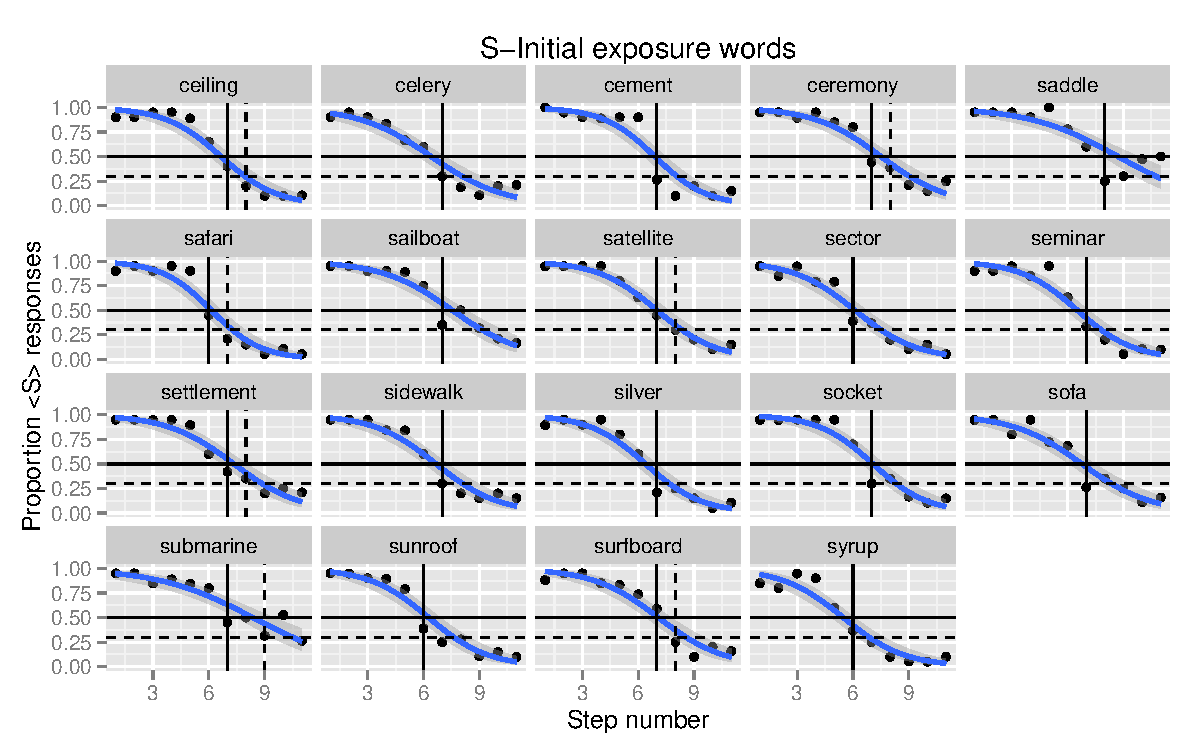
\includegraphics[width=\textwidth]{sinitialpretest.pdf}
\caption{Proportion of word-responses for /s/-initial exposure words. Solid lines represent Experiment 1 selection criteria (50\% word-response rate) and dashed lines represent Experiment 2 selection criteria (30\% word-response rate).  Dots are averaged word-response across subjects, and the blue line is a binomial model constructed from the responses.}
\end{figure}

The proportion of s-responses (or word responses for exposure items) at each step of each continuum was calculated and the most ambiguous step chosen. 
The threshold for the ambiguous step for this experiment was when the percentage of s-response dropped near 50\%. 
A full list of steps chosen for each stimulus item is in the appendix.  For the minimal pairs, six steps surrounding the 50\% cross over point were selected for use in the phonetic categorization task.  
Due to experimenter error, the continuum for \emph{seedling} was not included in the stimuli, so the chosen step was the average chosen step for the /s/-initial words.  
The average step chosen for /s/-initial words was 6.8 ($SD = 0.5$), and for /s/-final words the average step was 7.7 ($SD = 0.8$).

\begin{figure}[!ht]
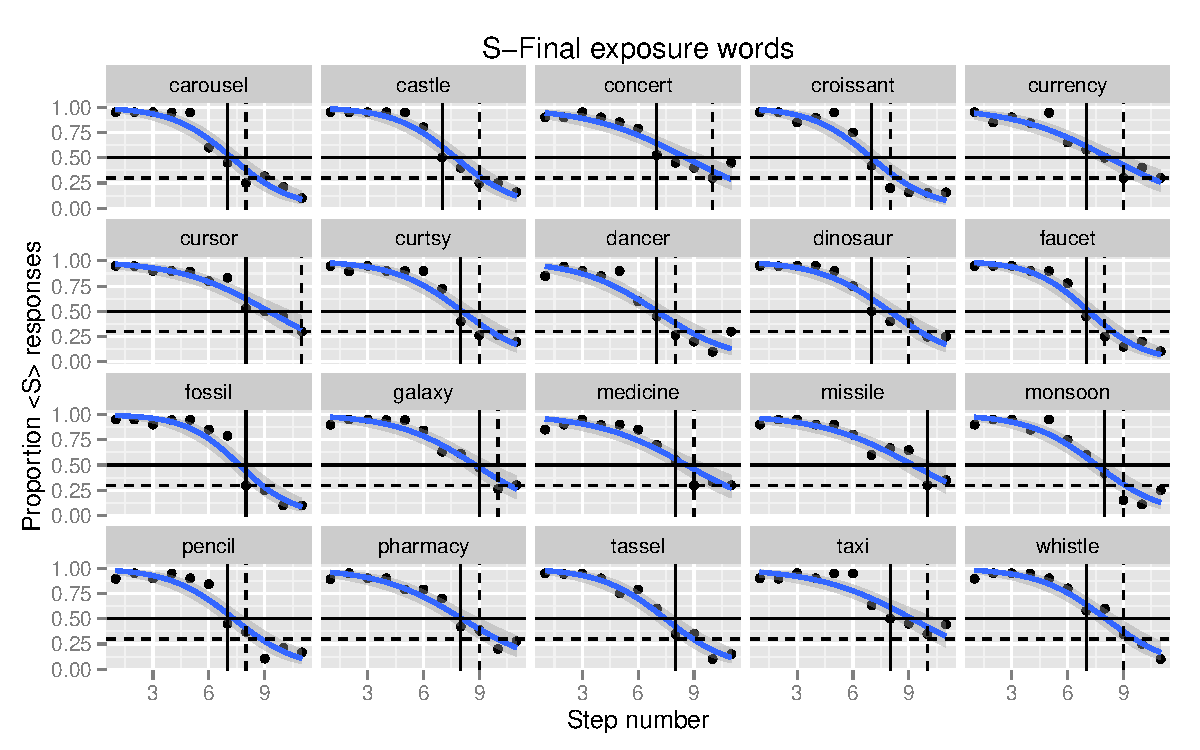
\includegraphics[width=\textwidth]{sfinalpretest.pdf}
\caption{Proportion of word-responses for /s/-final exposure words. Solid lines represent Experiment 1 selection criteria (50\% word-response rate) and dashed lines represent Experiment 2 selection criteria (30\% word-response rate).  Dots are averaged word-response across subjects, and the blue line is a binomial model constructed from the responses}
\end{figure}

\subsection{Procedure}

Participants in the experimental conditions completed two tasks, an exposure task and a categorization task.  
The exposure task was a lexical decision task, where participants heard auditory stimuli and were instructed to respond with either "word" if they thought what they heard was a word or "nonword" if they didn't think it was a word.  
The buttons corresponding to "word" and "nonword" were counterbalanced across participants. Trial order was pseudorandom, with no critical or control items appearing in the first six trials, and no critical or control trials in a row, but random otherwise, following \citet{Reinisch2013}.

In the categorization task, participants heard an auditory stimulus and had to categorize it as one of two words, differing only in the onset sibilant (s vs sh).  
The buttons corresponding to the words were counterbalanced across participants.  
The six most ambiguous steps of the minimal pair continua were used with seven repetitions each, giving a total of 168 trials.
Participants were instructed that there would two tasks in the experiment, and both tasks were explained at the beginning to remove experimenter interaction between exposure and categorization.  

Participants were assigned to one of four conditions. 
Two of the conditions exposed participants to only criticall items that began with /s/, and the other two exposed them to only critical items that had an /s/ in the onset of the final syllable, giving a consistent 200 trials in all exposure phases with control and filler items shared across all participants. 
Additionally participants in half the conditions received additional instructions that the speaker's "s" sounds were sometimes ambiguous, and to listen carefully to ensure correct responses in the lexical decision.

\bibliographystyle{apalike}
\bibliography{biblio}

\end{document}
